\documentclass{standalone}
\usepackage{tikz}
\begin{document}

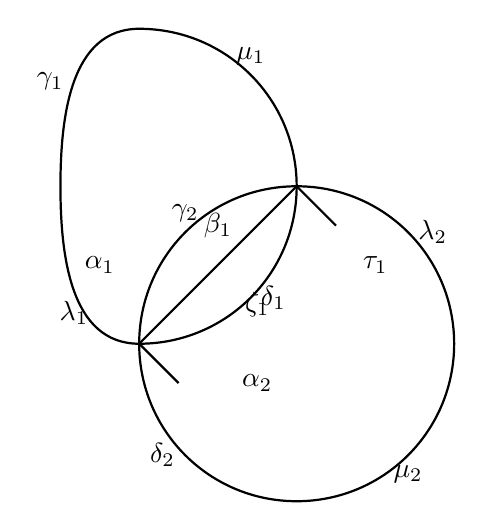
\begin{tikzpicture}

% First spherical linkage
\draw[thick]
    (0,0) 
    to[out=90,in=180] node[midway, left] {$\gamma_1$} 
    (1,2) 
    to[out=0,in=90] node[midway, above] {$\mu_1$} 
    (3,0) 
    to[out=-90,in=0] node[midway, right] {$\delta_1$} 
    (1,-2)
    to[out=180,in=-90] node[midway, below] {$\lambda_1$} 
    cycle;

% Second spherical linkage
\draw[thick]
    (3,0) 
    to[out=0,in=90] node[midway, right] {$\lambda_2$} 
    (5,-2) 
    to[out=-90,in=0] node[midway, below] {$\mu_2$} 
    (3,-4) 
    to[out=180,in=-90] node[midway, left] {$\delta_2$} 
    (1,-2)
    to[out=90,in=180] node[midway, above] {$\gamma_2$} 
    cycle;

% Gap and angles
\draw[thick] (1,-2) -- (3,0);
\draw[thick] (1,-2) -- (1.5,-2.5);
\draw[thick] (3,0) -- (3.5,-0.5);

% Labels
\node at (0.5,-1) {$\alpha_1$};
\node at (2,-0.5) {$\beta_1$};
\node at (2.5,-2.5) {$\alpha_2$};
\node at (4,-1) {$\tau_1$};
\node at (2.5,-1.5) {$\zeta_1$};

\end{tikzpicture}

\end{document}